\section{Method}\label{sec:method}
\begin{figure*}[t]
\centering
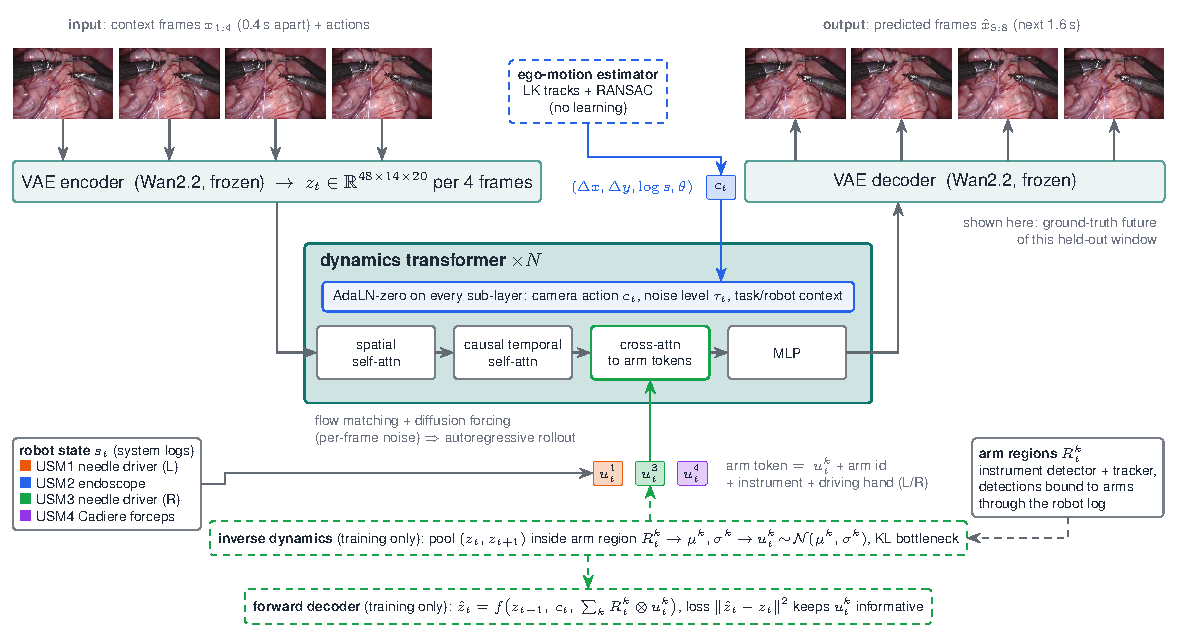
\includegraphics[width=\textwidth]{architecture.pdf}
\caption{\method{}. Context frames are encoded by a frozen video VAE; a latent spatio-temporal diffusion transformer predicts future latents conditioned on an explicit endoscope ego-motion action (through AdaLN) and on one token per robot arm (through cross-attention) that carries the arm's identity, its logged instrument and a latent action inferred from that arm's instrument region. In training only, a forward decoder predicts each latent from its predecessor and the actions placed on their regions, which keeps the learned actions informative. Sample input and output from a held-out test case.}
\label{fig:arch}
\end{figure*}

\subsection{Overview}
Let $x_{0:32}$ be 33 consecutive endoscopic frames (3.3\,s at 10\,fps) of the endoscope field, resized to $224\times320$. A frozen causal video VAE \cite{wan} maps them to latents $z_{0:8}$, $z_t\in\mathbb{R}^{48\times14\times20}$, where $z_0$ encodes $x_0$ and $z_t$ ($t\ge1$) encodes frames $4t-3,\dots,4t$. The world model predicts $z_{n:8}$ from context $z_{0:n-1}$, the robot state $s_t$ and an action $a_t$ for every transition $z_{t-1}\to z_t$:
\begin{equation}
a_t=\big(c_t,\ \{u^k_t\}_{k\in\mathcal{K}_t}\big),
\end{equation}
where $c_t$ is the endoscope ego-motion and $u^k_t$ a latent action for each arm $k$ that carries an instrument.

\subsection{Endoscope action}
The endoscope is an arm of the robot that the surgeon commands, so we treat its motion as an explicit action. For consecutive frames we track Shi--Tomasi corners \cite{shitomasi} with pyramidal Lucas--Kanade \cite{lucaskanade}, discard tracks failing a forward--backward check, and fit a similarity transform with RANSAC \cite{ransac}; instruments move independently of the camera and are rejected as outliers. Each transition yields $(\Delta x,\Delta y,\log s,\theta)$ with translations measured at the image centre as fractions of the frame size. Because the endoscope is still most of the time and then moves quickly, we compress each parameter with a signed logarithm $\operatorname{sign}(c)\log(1+|c|/\sigma)$, $\sigma$ being its 90th percentile. A fit is unreliable when fewer than 12 tracks survive or the RANSAC inlier ratio is below 0.5 (12\,\% of transitions); its parameters are set to zero and a validity flag is cleared, so that ``not measured'' is not confused with ``endoscope still''. The four transitions inside a latent step and their flags form $c_t\in\mathbb{R}^{20}$.

\textbf{Validation.} On CRCD \cite{crcd}, which records the endoscope arm's joints, the estimate detects real endoscope motion with a ROC AUC of 0.81 per latent step (0.88 on steps whose four transitions are all reliable); horizontal translation, vertical translation and scale correlate with the yaw, pitch and insertion joints ($r=0.63$, $0.70$, $0.42$; sign agreement 81, 87 and 73\,\%), and the joint motion predicts the estimate with a leave-one-episode-out $R^2$ of 0.41. These figures use only episodes whose video and kinematics we verified to be synchronized (Sec.~\ref{sec:setup}). On AutoLaparo \cite{autolaparo}, 300 clips of human laparoscopic hysterectomy with an assistant-held laparoscope in which surgeons labelled the laparoscope move beginning at 5\,s (static, up, down, left, right, zoom in or out), the motion measured in the following second separates moves from static clips with a ROC AUC of 0.87; a rule with five parameters fitted on the official training clips classifies the test clips with 71\,\% accuracy (majority class 22\,\%) and gives 81\,\% of the moves their correct direction, with signs that follow the camera geometry.

\subsection{Arm-bound instrument regions}
A YOLO11 detector \cite{yolo11} trained for SurgVU instrument detection locates instrument tips at the boundary frame of every latent step. Detections are bound to arms by solving, per frame, an assignment problem \cite{hungarian} between the arms that carry an instrument and the detections, with cost
\begin{equation}
C_{kj}=-\log p_j+\lambda_c\,\mathbb{1}[\hat y_j\neq o^k_t]+\lambda_s\,\lVert \mathbf{m}_j-\boldsymbol{\mu}^k\rVert_2,
\end{equation}
where $p_j$ and $\hat y_j$ are the detection's confidence and class, $\mathbf{m}_j$ its centre, and $\boldsymbol{\mu}^k$ the typical image position of arm $k$ in this case, estimated from frames in which every mounted instrument type is unique. Assignments above a cost threshold are rejected. The region $R^k_t$ of arm $k$ at step $t$ is the union of its boxes at the two boundary frames of the step, rasterized onto the $14\times20$ latent grid and dilated by one cell.

\subsection{Per-arm latent actions}
An inverse-dynamics model (IDM) infers each arm's action from the latents it moves. A small transformer encodes every latent position of the transition, $F=\mathrm{Trunk}([z_{t-1},z_t,z_t-z_{t-1}])$. A query built from the arm's identity and logged instrument attends to $F$ \emph{only inside} $R^k_t$, and a head outputs a diagonal Gaussian:
\begin{equation}
(\boldsymbol\mu^k_t,\log\boldsymbol\sigma^{2,k}_t)=g\big(\mathrm{Attn}(q(k,o^k_t),F;\,R^k_t)\big),\quad u^k_t\sim\mathcal{N}(\boldsymbol\mu^k_t,\boldsymbol\sigma^{2,k}_t),
\end{equation}
with $u^k_t\in\mathbb{R}^{8}$. A Kullback--Leibler penalty towards $\mathcal{N}(0,I)$ bounds the information each action carries; arms without a visible instrument receive $u^k_t=0$. Restricting the evidence to the arm's own region prevents an arm's action from describing endoscope motion or another instrument, and binding through the log gives every action a fixed physical meaning across cases.

\subsection{Dynamics transformer}
The dynamics model is a latent spatio-temporal diffusion transformer. Latent positions become tokens; each block applies self-attention within a frame with 2-D rotary embeddings \cite{rope}, causal self-attention across frames at each position, cross-attention to the arm tokens of the frame, and a SwiGLU MLP. Arm $k$ at step $t$ contributes the token
\begin{equation}
e^k_t=W_u u^k_t+E_{\mathrm{arm}}[k]+E_{\mathrm{occ}}[o^k_t]+E_{\mathrm{hand}}[h^k_t],
\end{equation}
where $h^k_t$ is the driving hand when the overlay shows it. The noise level and the endoscope action modulate every sub-layer through adaptive normalization with a shared projection and per-block offsets \cite{pixartalpha}.

\subsection{Training objective}
We train with rectified flow \cite{rectflow,flowmatching}. Every latent frame has its own noise level $\tau_t\in[0,1]$, $x_t=(1-\tau_t)z_t+\tau_t\epsilon_t$, and the network predicts the velocity $\epsilon_t-z_t$:
\begin{equation}
\mathcal{L}=\mathbb{E}\Big[\sum_{t}w_t\big\lVert v_\theta(x,\tau,a,s)_t-(\epsilon_t-z_t)\big\rVert^2\Big]+\lambda\,\mathcal{L}_{\mathrm{fwd}}+\beta\sum_{t,k}\mathrm{KL}\big(q(u^k_t)\,\Vert\,\mathcal{N}(0,I)\big).
\end{equation}
Trained on the diffusion loss alone, the learned actions collapse to the prior: in a pilot run all eight action dimensions became inactive (KL $0.004$\,nats per arm) and replacing every arm's action with another clip's changed the loss by less than $0.01$\,\%, while replacing the explicit endoscope action raised it by up to 14\,\%. Presumably the diffusion model explains most of a transition from its context frames and the noisy target, so the few nats an action carries are not worth their KL cost. We therefore add a latent-action-model objective as in \cite{genie,lapa,adaworld}, grounded like the actions themselves: a small convolutional decoder $f$ with a $9\times9$-cell receptive field predicts each latent from its predecessor, the endoscope action and the arm actions placed on their regions,
\begin{equation}
\mathcal{L}_{\mathrm{fwd}}=\sum_t\big\lVert f\big(z_{t-1},c_t,\textstyle\sum_k R^k_t\otimes u^k_t\big)-z_t\big\rVert^2,
\end{equation}
where $R^k_t\otimes u^k_t$ writes $u^k_t$ into the channels of arm $k$ at the positions of its region. Instrument motion cannot be predicted locally without the actions, which keeps them informative while the diffusion model learns to use them. In pilots on identical data, a weaker bottleneck alone kept six of the eight action dimensions active, but the diffusion model hardly used them; adding the decoder made all eight active and lowered the error of futures replayed from the inferred actions by 12\,\% (17\,\% inside the instrument regions). Baseline action interfaces receive the same decoder, with the monolithic or slot actions broadcast to every position. We use $\lambda=1$ and $\beta=10^{-4}$.
With probability 0.75 the first one to three latents are context ($\tau=0$, or $\tau\sim\mathcal{U}(0,0.1)$ to tolerate drift) and the remaining frames share one noise level or receive independent ones; otherwise all levels are independent, as in Diffusion Forcing \cite{dforcing}. Noise levels follow a logit-normal distribution \cite{sd3}, $w_t$ excludes context frames, and $\beta$ is ramped up over the first \num{10000} steps. With probability 0.1 all actions are dropped, which enables classifier-free guidance on actions.

\subsection{Inference}
Given context latents, future latents start from noise and are integrated with Euler steps from $\tau=1$ to $0$ while context latents stay fixed. Actions are either inferred from ground-truth video (\emph{action replay}, used to measure how well actions explain the future), taken from another clip (\emph{action swap}, to measure controllability), or set directly: an endoscope motion, or the action of a single arm. Longer rollouts re-anchor on the last generated frames.
